\documentclass{article}
 
% Required packages and libraries
\usepackage{circuitikz}
\usetikzlibrary{calc}
\usepackage{amsmath}
\usepackage{amssymb}
\usepackage{graphicx}


\title{CSSE2010 Course Notes}
\author{Paddy Maher}

\begin{document}
\maketitle
\newpage

\section{Introduction}
Following on from the lecture notes as prescribed by the CSSE2010 course, the course notes will be outputting through
looking at the levels of abstraction of a computer.

[insert graph of abstraction in computers]

\section{Digital logic level}

\subsection{Bytes and bits}

\begin{itemize}
\item Computers represent everything in \textbf{binary}
\item \textbf{Bit} = binary digit (0 or 1)
\item \textbf{Byte} = 8 bits
\item Modern computers deal with words which are usually a power of 2 number of bytes. For example:
\begin{itemize}
\item 1, 2, 4 or 8 bytes = 8, 16, 32 or 64 bits
\end{itemize}
\end{itemize}

\subsection{Representing whole unsigned numbers in binary}

\subsubsection{Conversion from binary to decimal and vice versa}

Converting binary to decimal
\begin{itemize}
\item Add values of each position where bit is 1
\item Example: 1010011 = 128 + 32 + 4 + 2 + 1 = 167
\end{itemize}

Converting Decimal to Binary \\

\textbf{Method 1}
\begin{itemize}
\item Rewrite '\textit{n}' as the sum of powers of 2 \textit{(by repeating subtracting largest powers of 2 not greater
than n)}
\item Assemble binary number from 1's in bit positions corresponding to those powers of 2, 0's elsewhere
\end{itemize}

\textbf{Method 2} \\ \\
Building up bits from the right (least significant bit \textit{(LSB}) to most \textit{(MSB}))
\begin{itemize}
\item Divide \textit{n} by 2
\item Remainder of division \textit{(0 or 1)} is next bit
\item Repeat with \textit{n} = quotient
\end{itemize}

\subsubsection{Least and Most Significant Bits}
The most significiant bit is denoted as \textbf{MSB}, likewise, the least significant bit is denoted as \textbf{LSB}.
These bits can be found on a binary number typically as the leftmost and rightmost bits respectively.

[arrow pointing to example of MSB and LSB in binary number]

\subsection{Basic Digital Logic}
\subsubsection{Digital circuits and Logic gates}

\underline{Digital Circuits}
\begin{itemize}
\item Only two logical levels present (i.e. binary)
\begin{itemize}
\item Logic '0'; usually small voltage \textit{(e.g. around 0 volts)}
\item Logic '1'; usually larger voltage \textit{(e.g. 0.8 to 5 volts, depending on the "logic family", i.e. type/size of
transistors)}
\end{itemize}
\end{itemize}

\underline{Logic gates}
\begin{itemize}
\item Are the building blocks of computers
\item Each gate has
\begin{itemize}
\item One or more inputs
\item Exactly one ouput
\end{itemize}
\item Perform logic operations \textit{or functions}
\begin{itemize}
\item 7 basic types: \textbf{NOT}, \textbf{AND}, \textbf{OR}, \textbf{NAND}, \textbf{NOR}, \textbf{XOR}
\textbf{XNOR}
\item Inputs and outputs can have only two states \textbf{1} and \textbf{0}; can be called "true" and "false"
respectively.
\item Logic symbol, truth table, boolean expression, timing diagram
\end{itemize}
\end{itemize}

\subsubsection{Basic Logic Gates}

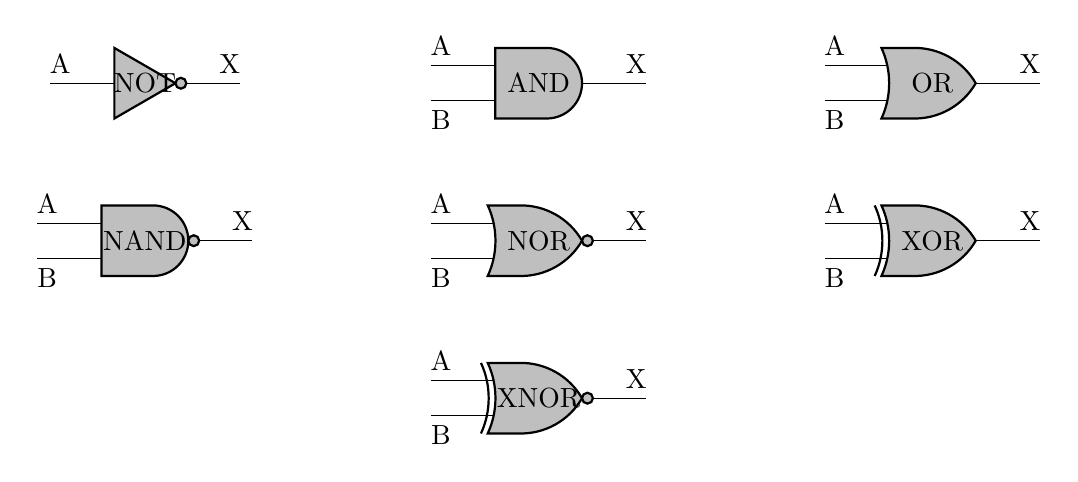
\begin{tikzpicture}
% Circuit style
\ctikzset{
    logic ports=ieee,
    logic ports/scale=0.8,
    logic ports/fill=lightgray
}
 
% Logic ports
\node[not port] (Noa) at (0,0){NOT};
\node[and port] (Anda) at (5,0){AND};
\node[or port] (Ora) at (10,0){OR};

\node[nand port] (Nanda) at (0,-2){NAND};
\node[nor port] (Nora) at (5,-2){NOR};
\node[xor port] (Xora) at (10,-2){XOR};

\node[xnor port] (Xnora) at (5,-4){XNOR};

% Connection 
\draw (Noa.in 1) -- ++(-.5,0)node[near end,above](In1){A};
\draw (Noa.out) -- ++(.5,0) node[near end,above]{X};

\draw (Anda.in 1) -- ++(-.5,0)node[near end,above](In1){A};
\draw (Anda.in 2) -- ++(-.5,0)node[near end,below](In1){B};
\draw (Anda.out) -- ++(.5,0) node[near end,above]{X};

\draw (Ora.in 1) -- ++(-.5,0)node[near end,above](In1){A};
\draw (Ora.in 2) -- ++(-.5,0)node[near end,below](In1){B};
\draw (Ora.out) -- ++(.5,0) node[near end,above]{X};

\draw (Nanda.in 1) -- ++(-.5,0)node[near end,above](In1){A};
\draw (Nanda.in 2) -- ++(-.5,0)node[near end,below](In1){B};
\draw (Nanda.out) -- ++(.5,0) node[near end,above]{X};

\draw (Nora.in 1) -- ++(-.5,0)node[near end,above](In1){A};
\draw (Nora.in 2) -- ++(-.5,0)node[near end,below](In1){B};
\draw (Nora.out) -- ++(.5,0) node[near end,above]{X};

\draw (Xora.in 1) -- ++(-.5,0)node[near end,above](In1){A};
\draw (Xora.in 2) -- ++(-.5,0)node[near end,below](In1){B};
\draw (Xora.out) -- ++(.5,0) node[near end,above]{X};

\draw (Xnora.in 1) -- ++(-.5,0)node[near end,above](In1){A};
\draw (Xnora.in 2) -- ++(-.5,0)node[near end,below](In1){B};
\draw (Xnora.out) -- ++(.5,0) node[near end,above]{X};
\end{tikzpicture}

\subsection{Boolean Logic}
\subsubsection{Boolean Logic Functions}
\begin{itemize}
\item Logic functions can be expressed as expressions involving:
\begin{itemize}
\item variables \textbf{(literals)}, e.g A, B, X
\item functions, e.g +, ., $\oplus$, $\overline{X}$
\end{itemize}
\item Rules about how this works are called \textbf{Boolean algebra}
\item Variables and functions can only take on values 0 or 1
\end{itemize}

\subsubsection{Boolean Algebra conventions}

\underline{Conventions}
\begin{itemize}
\item Inverstion: [insert overline] (overline)
\begin{itemize}
\item e.g. NOT(A) = $\overline{A}$ \textit(A bar)
\end{itemize}

\item AND: dot( . ) or implied \textit(by adjacency)
\begin{itemize}
\item e.g. AND(A,B) = AB = A.B
\end{itemize}

\item OR: plus sign (+)
\begin{itemize}
\item e.g. OR(A,B,C) = A+B+C
\end{itemize}
\end{itemize}

\underline{Other examples}
\begin{itemize}
\item XOR(A,B) = A $\oplus$ B = $\overline{A}$B + A$\overline{B}$
\item NAND(A,B,C) = $\overline{ABC}$
\item NOR(A,B) = $\overline{A+B}$
\end{itemize}

\subsubsection{Summary of logic function representations}
There are four representations of logic functions \textit{(assume function of \textbf{n} inputs)}

\begin{itemize}
\item{Truth}
\begin{itemize}
\item Lists output for all $2^n$ combinations of inputs (Best to list inputs in a systematic way)
\end{itemize}

\item{Boolean function (or equation)}
\begin{itemize}
\item Describes the conditions under which the function output is 1 
\end{itemize}

\item{Logic Diagram}
\begin{itemize}
\item Combination of logic symbols joined by wires
\end{itemize}

\item{Timing Diagram}
\end{itemize}

\subsubsection{Logic function implementation}

\begin{itemize}
\item Any logic function can implemented as the \textbf{OR} of \textbf{AND} combinations of the inputs
\begin{itemize}
\item Called 'sum of products'
\end{itemize}

\item{Example:}
\begin{itemize}
\item Consider truth table
\begin{tabular}{ c| c| c| c }
 A & B & C & M \\ 
 \hline
 0 & 0 & 0 & 0 \\  
 0 & 0 & 1 & 0 \\  
 0 & 1 & 0 & 0 \\  
 0 & 1 & 1 & 1 \\  
 1 & 0 & 0 & 0 \\  
 1 & 0 & 1 & 1 \\  
 1 & 1 & 0 & 1 \\  
 1 & 1 & 1 & 1 \\  
\end{tabular}
\item For each '1' in the output column, write down the \textbf{AND} combination of inputs that give 1
\item \textbf{OR} these together
\end{itemize}
\end{itemize}

\underline{Equivalent functions}
\begin{itemize}
\item Sum of products does not necessarily produce circuit with minimum number of gates
\item Can '\textit{manipulater}' boolean functions to give an equivalent function
\begin{itemize}
\item Use rules of boolean algebra
\end{itemize}
\item Example: \textbf{Z} = \textbf{AB} + \textbf{AC} = \textbf{A}(\textbf{B}+\textbf{C})
\end{itemize}

\underline{Boolean identities} \\ \\
\begin{tabular}{l|l|l}
Name & \textbf{AND} form & \textbf{OR} form \\
\hline
Identity law & 1\textbf{A} = \textbf{A} & 0 + \textbf{A} = \textbf{A} \\
Null law & 0\textbf{A} = \textbf{A} & 1 + \textbf{A} = 1 \\
Idempotent law & \textbf{AA} = \textbf{A} & \textbf{A} + \textbf{A} = \textbf{A} \\
Inverse law & \textbf{A$\overline{A}$} = 0 & \textbf{A} + $\overline{\textbf{A}}$ = 1 \\
Commutative law & \textbf{AB} = \textbf{BA} & \textbf{B} + \textbf{A} = \textbf{B} + \textbf{A} \\
Associative law &(\textbf{AB})\textbf{C} = \textbf{A}(\textbf{BC}) & (\textbf{A} + \textbf{B}) + \textbf{C} = \textbf{A} + 
(\textbf{B} + \textbf{C}) \\
Distributive law & \textbf{A}+\textbf{BC} = (\textbf{A+B})\textbf{.}(\textbf{A+C}) & \textbf{A.}(\textbf{B} + \textbf{C}) = \textbf{AB} + \textbf{AC} \\
Absorption law & \textbf{A}(\textbf{A+B}) = \textbf{A} & \textbf{A} + \textbf{AB} = \textbf{A}\\
De Morgan's law & $\overline{\textbf{AB}}$ = $\overline{\textbf{A}}$ + $\overline{\textbf{B}}$&
$\overline{\textbf{A}}$ + $\overline{\textbf{B}}$ = $\overline{\textbf{AB}}$ 
\end{tabular}

\subsubsection{Number bases}
[Flow diagram of Binary(base 2), Decimal(base 10), Hex(base 16), Octal(base 8)]
[May need to add further details of the table (in regard to the individual binary representations)]

\begin{tabular}{ c | c | c | c | c | c }
\hline
\textbf{MSB} &  &  &  &  \textbf{LSB} &  \\
$2^(n-1)$ & $2^(n-2)$ & .. & $2^1$ & $2^0$ & Excess-$2^(n-1)$ ; $-2^(n-1) \leq$ x $\leq (2^(n-1)-1)$ \\
$-2^(n-1)$ & $2^(n-2)$ & .. & $2^1$ & $2^0$ & 2's comp ; $-2^(n-1) \leq$ x $\leq (2^(n-1)-1)$ \\
$-2^(n-1)-1$ & $2^(n-2)$ & .. & $2^1$ & $2^0$ & 1's comp ; $-(2^(n-1)-1) \leq$ x $\leq (2^(n-1)-1)$ \\
+/- & $2^(n-2)$ & .. & $2^1$ & $2^0$ & Sign-Mag ; $-(2^(n-1)-1) \leq$ x $\leq (2^(n-1)-1)$ \\
$2^(n-1)$ & $2^(n-2)$ & .. & $2^1$ & $2^0$ & Unsigned ; $0 \leq$ x $\leq 2^n-1$ \\
\end{tabular}
[fix peculiar exponential  layout]

\subsubsection{Equivalent Circuits}
\begin{itemize}
\item All circuits can be constructed from \textbf{NAND} or \textbf{NOR} gates
\begin{itemize}
\item These are called 'complete' gates
\end{itemize}

\item{Examples:}
[insert NOT AND OR logic gates]

\item Reason: Easier to build \textbf{NAND} and \textbf{NOR} gates from transistors
\end{itemize}

\subsection{Binary Arthmetic}

\subsubsection{Binary addition}

\begin{itemize}
\item{Addition is quite simple in binary}
\item
\begin{tabular} { l | c c c c}
Addend & 0 & 0 & 1 & 1 \\
Augend & 0 & 1 & 0 & 1 \\
 & 0 & 1 & 1 & 0 \\
 & 0 & 0 & 0 & 1 
\end{tabular}
\item Above ignores carry in
\end{itemize}
[make sense of the table above]

\begin{tabular} { r | c | r | c }
Decimal & 8-bit unsigned & Decimal & 2's complement \\
10 & 00001010 & 10 & 00001010 \\
+ 243 & + 11110011 & + (-13) & + 11110011 \\
\hline
253 & 11111101 & -3 & 11111101 \\
\end{tabular}

\begin{itemize}
\item Format matters upon interpreting the number
\item Whatever the format is the bit-wise addition (which leads to the hardware circuit) is the same.
\item Two's complement; there is no need to do anything with the carry out from the \textbf{MSB} to get the correct result
\item But in one's complement, the carry out from the MSB will have to be added back to the result to get the correct answer;
this is one drawback of one's complement representation

\underline{Overflow in binary addition}

\begin{tabular} { r | c | r | c }
Decimal & 8-bit unsigned & Decimal & 2's complement \\
15 & 00001111 & 125 & 01111101 \\
+ 243 & + 11110011 & + 4 & + 00000100 \\
\hline
258 & 00000010 & 129 & 10000001 \\
\end{tabular}

Overflow: Not enough bits to represent the answer. The result goes out of range thus outputting an incorrect answer.

\begin{itemize}
\item Unisgned: carry-out from the \textbf{MSB} $\rightarrow$ overflow
\item 2's comp: carry-in to the \textbf{MSB} and carry-out from the \textbf{MSB} are different $\rightarrow$ overflow
\item Equivalently, overflow occurs if (in 2's comp)
\begin{itemize}
\item Two negatives added together give a positive, or;
\item Two positives added together give a negative
\end{itemize}
\end{itemize}

\subsubsection{Adders and addition of binary words}

A device which adds 2 bits \textit{(with no carry-in)} is called a 'half-adder'
[insert half adder diagrams]

\underline{Addition of binary words}

\item Have to be able to deal with carry-in
\item 
\begin{tabular}{ c c c c c }
A & B & Cin & Cout & Sum \\ 
\hline
 0 & 0 & 0 & 0 & 0 \\  
 0 & 0 & 1 & 0 & 1 \\  
 0 & 1 & 0 & 0 & 1 \\  
 0 & 1 & 1 & 1 & 0 \\  
 1 & 0 & 0 & 0 & 1 \\  
 1 & 0 & 1 & 1 & 0 \\   
 1 & 1 & 0 & 1 & 0 \\  
 1 & 1 & 1 & 0 & 1 \\   
\end{tabular}
\item \textbf{S} = $\overline{\textbf{AB}}$C + $\overline{\textbf{A}}$\textbf{B}$\overline{\textbf{C}}$ + ...
\item \textbf{S} = \textbf{A} $\oplus$ \textbf{B} $\oplus$ \textbf{Cin}
\end{itemize}


[insert full adder diagram with relevant sum and carry-out equation]

\underline{Binary Adder}
\begin{itemize}
\item Can cascade full adders to make binary adder
\begin{itemize}
\item Example: for 4 bits ...
[insert 4 bit binary adder diagram]
\end{itemize}
\item This is a ripple-carry adder
\end{itemize}

\subsubsection{Binary subtraction}
\begin{itemize}
\item \textbf{A} - \textbf{B}; usually implemented as \textbf{A} + (-\textbf{B})
\begin{itemize}
\item \textbf{A} and \textbf{B} are multi-bit quantities
\item '\textit{+}' in this case means addition (not \textbf{OR})
\item -\textbf{B} means negative \textbf{B} - the two's complement of \textbf{B}
\end{itemize}
\item Two's complement of \textbf{B} can be calculated by flipping bits and adding 1.
\end{itemize}

[add relevant equations and interpretations]

How can one use a gate to flip a bit, but only somtimes? i.e
\begin{itemize}
\item \textbf{Z} = NOT(\textbf{B}) when \textbf{M} is 1
\item \textbf{Z} = \textbf{B} when \textbf{M} is 1
\end{itemize}

\subsubsection{Adder-subtractor}

[insert image]

\textbf{M} = carry-in

\subsection{Combinational Circuits}
\begin{itemize}
\item Generally, n inputs $\rightarrow$ m outputs [insert image of combinational circuit]
\item Each output can be expressed as a function of \textit{n} input variables
\item Output depends on current inputs only
\item Can write truth table also:
\begin{itemize}
\item \textit{n} input columns
\item \textit{m} output columns
\item $2^{n}$ rows \textit{(i.e. possible input combinations)}
\end{itemize}
\end{itemize}

\subsubsection{Multiplexer \textit{(or Mux)}}

\begin{itemize}
\item $2^{n}$ data inputs
\item 1 output
\item \textit{n} control (or select) inputs- that select one of the inputs to be \textit{"sent"} or \textit{"steered"} to the output
\item Example: 4-to-1 multiplexer [insert image of logical symbol for multiplexer] \\
\begin{tabular}{ c c c }
$S_{1}$&$S_{0}$&F\\
0&0&$D_{0}$\\
0&0&$D_{0}$\\
0&0&$D_{0}$\\
0&0&$D_{0}$\\
\end{tabular}
\end{itemize}

[insert 4-to-1 Multiplexer Logic Circuit Implementation]

\subsubsection{Decoder}

Decoder
\begin{itemize}
\item Converts \textit{n}-bit input to be a logic-1 on exactly one of $2^{n}$ outputs
\item Example 3-to-8 decoder \\
\begin{tabular}{ c c c | c c c c c c c c }
A & B & C & $D_{0}$ & $D_{1}$ & $D_{2}$ & $D_{3}$ & $D_{4}$ & $D_{5}$ & $D_{6}$ & $D_{7}$ \\
0 & 0 & 0 & 1 & 0 & 0 & 0 & 0 & 0 & 0 & 0 \\
0 & 0 & 1 & 0 & 1 & 0 & 0 & 0 & 0 & 0 & 0 \\
0 & 1 & 0 & 0 & 0 & 1 & 0 & 0 & 0 & 0 & 0 \\
0 & 1 & 1 & 0 & 0 & 0 & 1 & 0 & 0 & 0 & 0 \\
\end{tabular}
\textit{n} : $2^{n}$ decoder
\end{itemize}

\subsubsection{Gates aren't perfect}
Gates aren't perfect.. The reality of timing
[insert gates]
\begin{itemize}
\item Propagation delay- time for change in input to affect output
\item Fall time- time taken for output to fall from 1 to 0
\item Rise time- time for output to rise from 0 to 1
\end{itemize}

\subsection{Recap of Week 2}
\begin{itemize}
\item Combinational Logic Circuits- Adder, Adder/Subtractor, Multiplexer, Decoder
\item Logic Gates- \textbf{NOT}, \textbf{AND}, \textbf{OR}, \textbf{NAND}, \textbf{NOR}, \textbf{XOR}, \textbf{XNOR},
and Boolean algebra
\item Binary representations- assigned, signed-mag, 1's comp, 2's comp, excess-$2^{n-1}$
\end{itemize}

\subsubsection{Circuits that remember values}
\begin{itemize}
\item The output of any logic gate or \textit{'combinational circuit'} is dependent on the current value of inputs only
\item If an input changes, the output can also change and the previous value is lost forever
\item Sequential circuits: the current output depends not only on the current inputs but also on the past outputs
\item Circuits with memory can remember values, even if the input changes
\end{itemize}

Memory element: \underline{D Flip Flop}
\begin{itemize}
\item \textbf{D} is input
\item \textbf{Q} is output
\item \textbf{CLK} \textit{(clock)} is control input
\item How does it work
\begin{itemize}
\item \textbf{Q} copies the value of \textbf{D} (and remember it) whenever \textbf{CLK} goes from 0 to 1 (rising edge)
\end{itemize}
\end{itemize}

[insert logic time graphs of D, CLK, Q and logical symbols]

\subsubsection{Characteristic Tables}
\begin{itemize}
\item 'Characteristic table' defines operation of flip-flop in tabular form
\item D flip-flop
\begin{tabular}{ c | c }
\textbf{D} & \textbf{Q}(t+1) \\
0 & 0 \\
1 & 1 \\
\end{tabular}
\end{itemize}

\subsubsection{D Flip-flops}
\begin{itemize}
\item Summary: D flip-flops remember either a "1" to "0" ~ i.e a single bit. That is the flip-flop remember the value till the next clock edge, upon which the D input is transformed to output Q
\item To rmemeber 'n bits'
\item Definition: A n-bit register can be made using \textit{n} D flip-flops
\item There are other types of flip-flops, e.g.
\begin{itemize}
\item \textbf{JK} flip-flops
\item \textbf{T} flip-flops
\end{itemize}
\item Flip-flops can be made out of logic gates
\end{itemize}

\subsubsection{SR Latch}

[insert logic image of SR Latch]

\begin{itemize}
\item A \textbf{NOR} gate
\begin{tabular}{ c c c }
A & B & \textbf{NOR} \\
0 & 0 & 1 \\
0 & 1 & 0 \\
1 & 0 & 0 \\
1 & 1 & 0 \\
\end{tabular}
\item 
\begin{tabular} { c c c c }
S & R & Q & $\overline{Q}$ \\
0 & 0 & $Q_{k-1}$ & $\overline{Q}_{k-1}$ \\
0 & 1 & 0 & 1 \\
1 & 0 & 1 & 0 \\
1 & 1 & 0 & 0 \\
\end{tabular}
\end{itemize}

\subsubsection{Flip-flops vs Latches}
\begin{itemize}
\item Latches are level triggered devices- i.e. able to latch the output and respond to changes of logic levels on the inputs
\item Latch circuits can be modified such that they become sensitive to an edge \textit{(i.e momentary transitions)} of a control
input \textit{(i.e a clock signal)}
\item Such circuits are called "flip-flops" and a flip-flop can store one bit of information while being sensitive to a clock edge 
\textit{(i.e a flip-flop will change its output only at the clock edges, based on the inputs)}
\item A clock signal has two edges
\begin{itemize}
\item Positive edge- 0 to 1 transition
\item Negative edge- 1 to 0 transition
\end{itemize}
\item There are different types of flip-flops
\begin{itemize}
\item\textbf{D} flip-flop
\item \textbf{JK} flip-flop
\item \textbf{T} flip-flop
\end{itemize}
\item So, a \textbf{D} flip-flop can be positive edge triggered or negative edge triggered
\item Positive edge triggered \textbf{D} flip-flop $\rightarrow$ input \textbf{D} is copied to output \textbf{Q} at the positive edge of the clock. In between the clock edges, the flip-flop is non-reponsive, thus stores the value
\end{itemize}

[insert symbolic image of 'real D flip-flop]

\subsubsection{D Latches and Flip-flops- Symbols used}
[insert 4 images of latches and flip-flops]
\begin{itemize}
\item Triangle indicates edge-triggered \textit{(therefore flip-flop)}
\begin{itemize}
\item \textit{(c)} sensitive to rising edge of click
\item \textit{(d)} to falling edge
\end{itemize}
\item \textit{'State'} of a flip-flop is the value stored
\item Flip-flops are generally more useful than latches
\end{itemize} 

\underline{D Flip-flop chips}
\begin{enumerate}
\item \textbf{74HCT74} chip; Dual \textbf{D} flip-flop
\item \textbf{74HCT273} chip; eight \textbf{D} flip-flops
\begin{itemize}
\item can hold one byte of information \textit{(8 bits)}
\end{itemize}
\end{enumerate}

\subsection{Combinational vs Sequential Circuits}
\begin{itemize}
\item Combinational circuits
\begin{itemize}
\item Logic gates only
\end{itemize}
\item Output is uniquely determined by the inputs
\begin{itemize}
\item i.e: one will always get the same output for a given set of inputs
\end{itemize}
\item Example of a combinational circuit [insert this]
\item Sequential Circuits
\begin{itemize}
\item Include flip-flops
\item Output determined by current inputs and current 'state'
\item Output can only change when clock 'ticks'
\end{itemize}
\end{itemize}

\subsubsection{Sequential Circuits}
\begin{itemize}
\item 'State' = value stored in flip-flops
\item Output depends on input and state
\item Next state depends on input and state
[insert sequential circuit picture]
\end{itemize}

\subsubsection{Synchronous Sequential Circuit}
\begin{itemize}
\item Storage elements (flip-flops) can only change at discrete instants of time
\item Assume:
\begin{itemize}
\item There is a clock signal
\item Output of storage elements change only on the edges of control siganl
\begin{itemize}
\item \textit{(compare with logic gates whose output changes whenever the input changes)}
\end{itemize}
\end{itemize}
\end{itemize}

\underline{Registers}
\begin{itemize}
\item A \textit{register} is a group of flip-flops
\begin{itemize}
\item n-bit register consists of \textit{n} flip-flops capable of storing \textit{n} bits
\end{itemize}
\item A register is a sequential circuit without any combinational logic
\end{itemize}

\section{Microarchitecture level}

\section{Instruction set architecture level}

\section{Assembly language level}

\section{Problem-oriented language level}



\end{document}
